\chapter{Codec}
\label{cap:codec}
\section{Introduzione}
Il paradigma di protocollo di streaming a descrittori multipli rende
necessaria la progettazione di codec su misura. Viene rimandata al paragrafo
\ref{cap:implementazione_codec} la presentazione, a titolo esplicativo, del
\emph{codec testuale}.

\subsection{Caratteristiche del codec}
Affinché un codec possa funzionare con il protocollo MDC (\emph{Multiple
Description Coding}) è necessario che possieda delle caratteristiche ben precise.
La codifica MDC ha come obiettivo finale la descrizione di un file in modo tale
che, in caso di perdita parziale dei dati che lo costituiscono, il file stesso
sia ugualmente interpretabile. L'assoluta interpretabilità del file costituisce
un vincolo molto stringente e si rendono necessari codec progettati con
particolari accorgimenti. MDSP versione 0.1 gestisce file di tipo testuale e
immagini, consente di visualizzare il contenuto di un file anche se si verificano
errori nel trasferimento dello stesso attraverso una rete di telecomunicazioni.
Durante la fase di codifica il file sorgente viene suddiviso in descrizioni e
descrittori:
\begin{itemize}
 \item Un descrittore è la più piccola unità di misura del contenuto di un
 file. L'insieme di più descrittori costituisce una descrizione.
 \item Una descrizione può contenere parte o tutte le informazioni di un file
 (con `informazioni' si intendono i dati costituenti il file).
\end{itemize}
Le descrizioni costituiscono differenti codifiche e devono essere il più possibile ortogonali fra loro, in modo da poter essere indipendenti l'una dall'altra, pur riferendosi tutte allo stesso file sorgente.

Nel caso in cui qualche descrizione venga persa, sia corrotta, o non venga
inviata dalla sorgente, sarà comunque possibile decodificare il file ed
otterene un output sufficientemente corretto, tale da poter essere intepretato. \`E sufficiente la ricezione di una sola descrizione per la corretta ricostruzione del file sorgente. La ricezione di due o più descrizioni migliora l'accuratezza del file decodificato. Il file sorgente viene `\emph{descritto}' con più precisione.  Tale risultato viene raggiunto grazie alla creazione di codec che tengono in considerazione il fattore umano nell'interpretazione di vari tipi di informazioni:
\begin{itemize}
 \item Nel caso del testo, una parola con una lettera mancante viene facilmente interpretata dal lettore. Il cervello umano sostituisce la lettera mancante con quella corretta basandosi sul senso della parola stessa o della frase.
 \item Nel caso delle immagini, la mancanza di pixel non rende l'immagine inutilizzabile. All'occhio umano saranno presenti delle lievi alterazioni, ma, anche questa volta, il contesto rende ugualmente interpretabile l'immagine e le informazioni che essa contiene.
\end{itemize}

\begin{figure}[ht]
\centering 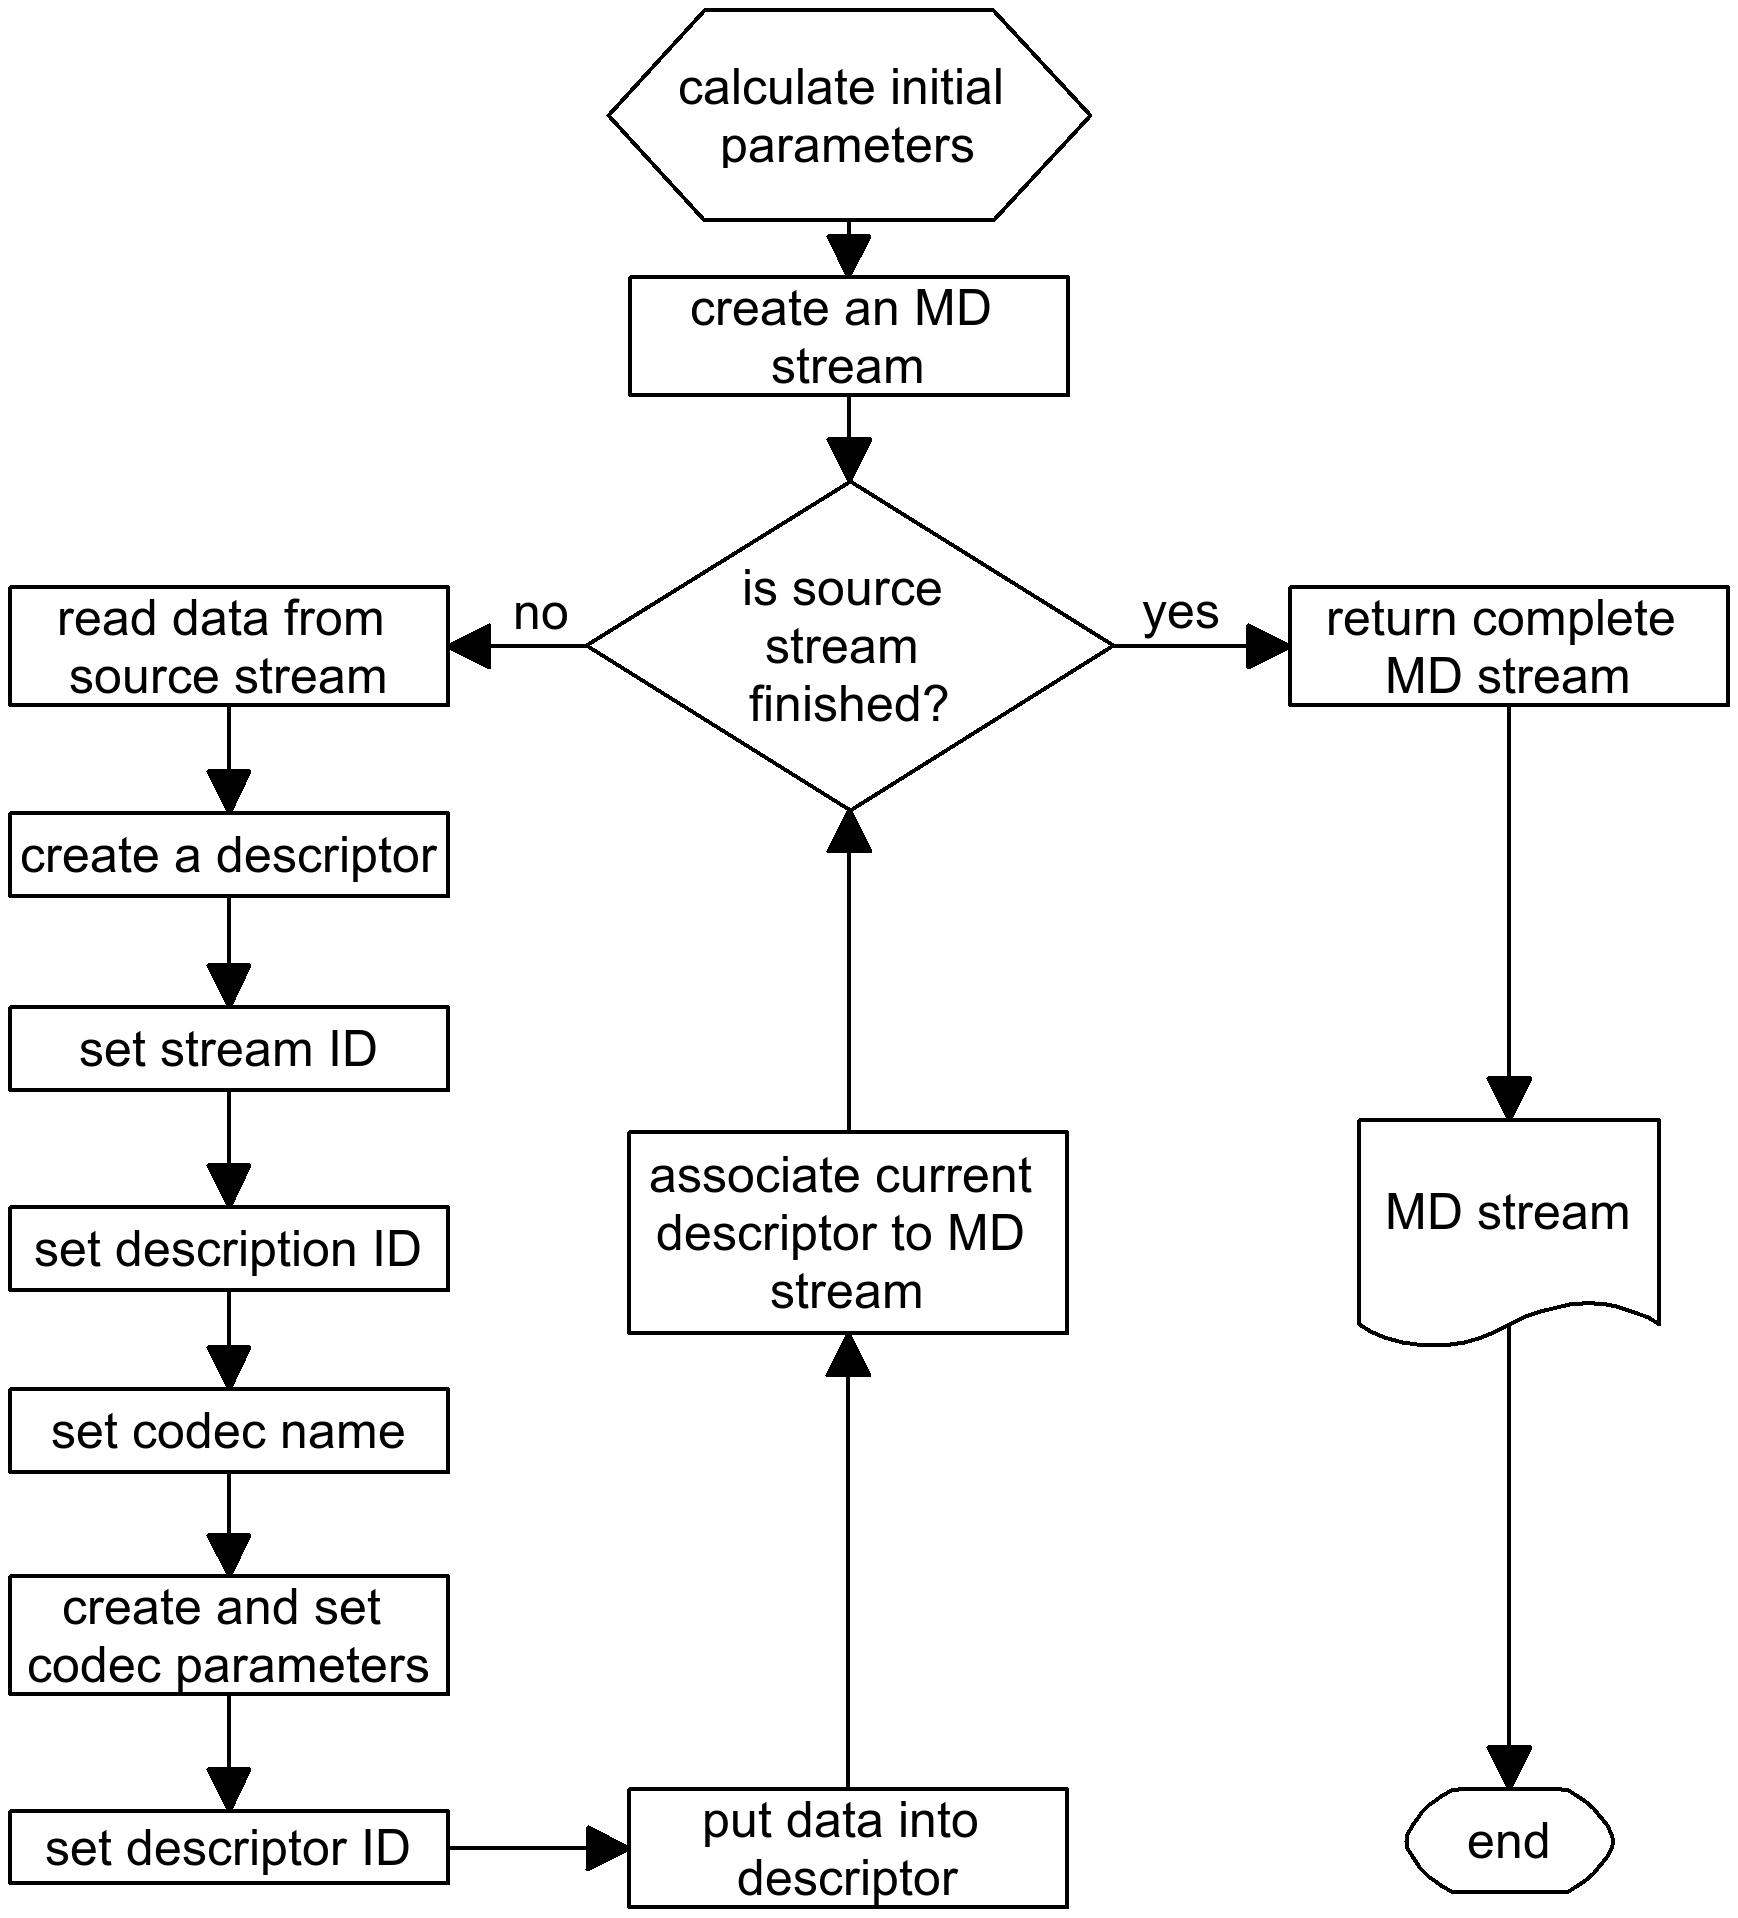
\includegraphics[width=0.90\textwidth]{../images/codifica.png}
	\caption{Diagramma di flusso dell'algoritmo di codifica.}
	\label{fig:codifica}
\end{figure}

\begin{figure}[ht]
\centering 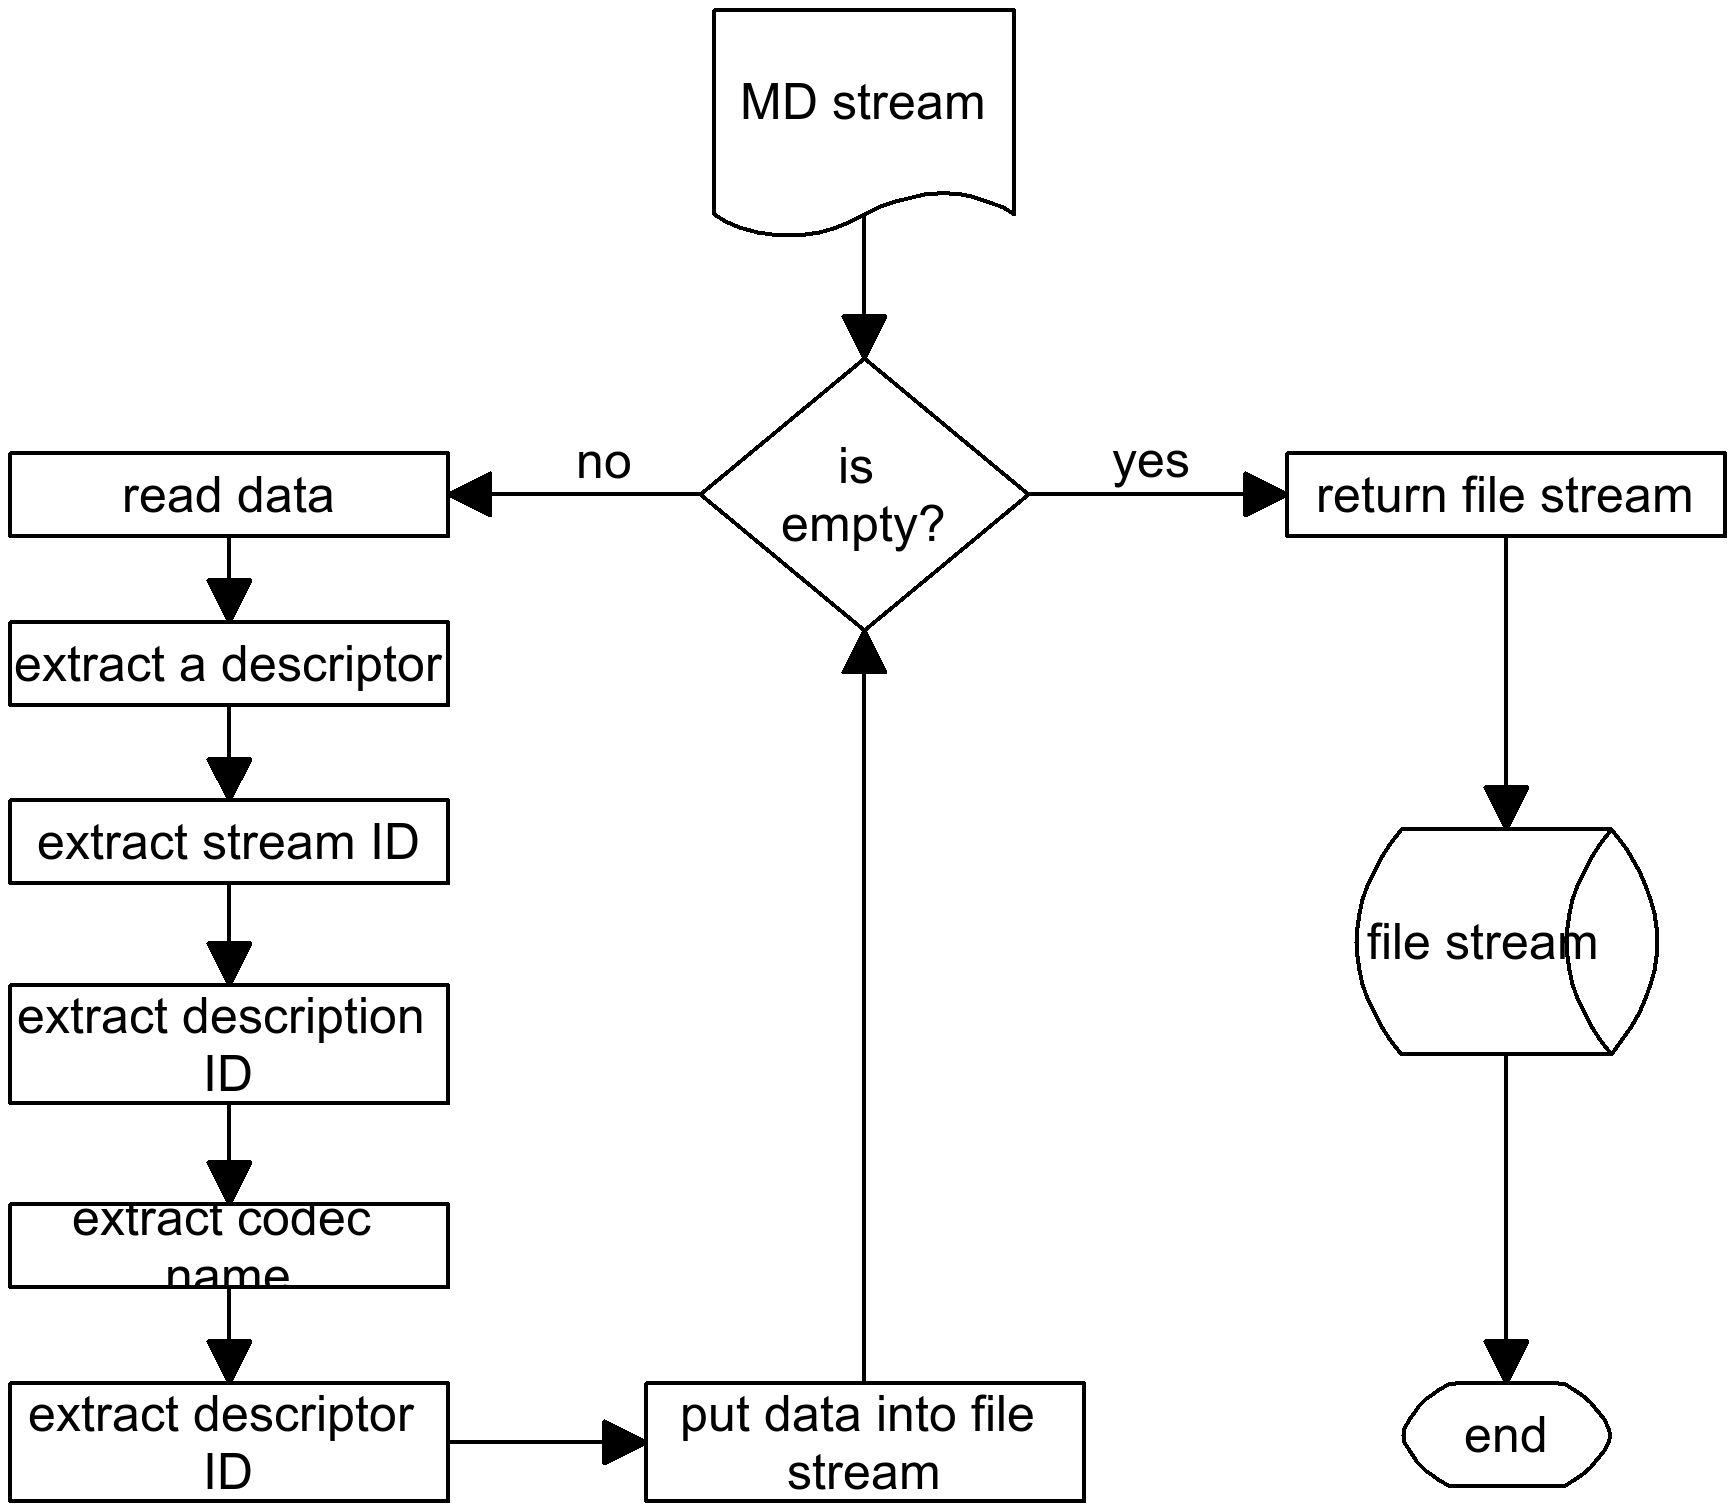
\includegraphics[width=0.90\textwidth]{../images/decodifica.png}
	\caption{Diagramma di flusso dell'algoritmo di decodifica.}
	\label{fig:decodifica}
\end{figure}

Il funzionamento del codec (illustrato in figura \ref{fig:codifica} e
\ref{fig:decodifica}) si può applicare per descrivere la suddivisione di ogni
descrizione in descrittori. Come accennato, i descrittori sono la più piccola unità di memorizzazione dei dati costituenti il file sorgente. Tale
affermazione significa che, se viene perso un descrittore durante il
trasferimento, oppure i suoi dati non sono corretti, esso può essere
semplicemente non considerato. Ciò permette un'estrema flessibilità di
decodifica. Sostanzialmente, il decodificatore deve adattarsi alla tipologia e
quantità di dati collezionati e creare un file di output. Tale file sarà perfetto se non si sono verificate perdite, o ugualmente interpretabile in presenza di perdite.


\section{Implementazione Codec}
\subsection{Codec testuale}
\label{cap:implementazione_codec}
Nel presente capitolo verrà descritto il funzionamento e l'implementazione
del codec testuale. L'analisi inizia da alcune considerazioni preliminari sul
file sorgente riguardanti la suddivisione delle informazioni secondo le
caratteristiche tipiche delle tecniche a descrizione multipla. Nella
implementazione di MDSP un file sorgente può essere suddiviso in uno o più
descrizioni, fino a un massimo di 64. Ogni descrizione, considerata
singolarmente, è in grado di descrivere l'intero file. \`E cioé sufficiente
alla corretta decodifica del file sorgente. Qualora il file sorgente venga
codificato in più di una descrizione sarà possibile la ricostruzione
perfetta del file esclusivamente nel caso in cui tutti le descrizioni giungano
a destinazione. Durante la procedura di decodifica del testo, MDSP versione 0.1
sostituisce un carattere \emph{spazio} qualora una lettera non giunga a
destinazione. Nel caso della decodifica di immagini viene sostituito il
pixel non giunto a destinazione con uno apportunamente scelto e
poi interpolato. Oltre tali accorgimenti, è necessario prendere in
considerazione l'eventualità che giunga a destinazione una singola descrizione
con alcuni descrittori errati (caso peggiore). Tale eventualità si risolve
facendo sì che durante la codifica i descrittori, ma ancor più le descrizioni,
contengano dati provenienti 'da tutte le zone del file'. Al fine del
raggiungimento di tale scopo, vengono di seguito riportati gli indici necessari
e alcune semplici formule per poterli colcolare:
\begin{itemize}
 \item Dimensione di ogni descrizione: $$\frac{dimensione\_file}{numero\_descrizioni}$$
 \item Numero di descrittori per ogni descrizione: $$\frac{dimensione\_descrizione}{dimensione\_descrittore}$$
 \item Dimensione di ogni descrittore: $$\frac{dimensione\_descrizione}{numero\_descrittori}$$
\end{itemize}
Tali accorgimenti non sono da soli sufficienti per la realizzazione di un codec
pienamente compatibile MDC, ulteriori accorgimenti verranno illustrati con
maggiore dettaglio nel paragrafo \ref{sec:esempio_codec}.

La struttura delle classi C++ di gestione dei codec comprende classi astratte
che regolano lo scambio di dati tra i codec e il motore di streaming, nonché la
composizione delle strutture dati in memoria da utilizzare. Le classi a cui ci
si riferisce sono contenute nella directory \texttt{mdc/src/codecs/}. Di seguito vengono elencate e brevemente descritte le classi astratte per la
gestione dei codec:
\begin{itemize}
 \item \textit{abstract\_codec\_parameter.h}: astrae i parametri del codec; per
 utilizzare tale classe è necessario specificare il comportamento di essa nelle
 funzioni \texttt{serialize()} e \texttt{deserialize()}.
 \item \texttt{abstract\_md\_codec.h}: astrae il funzionamento del codec a
 descrizioni multiple; per utilizzare tale classe è necessario specificare il
 comportamento di essa nelle funzioni \texttt{code()} e \texttt{decode()}. In
 tali funzioni è contenuto il cuore del codec e pertanto necessitano un'analisi
 più dettagliata, si rimanda al paragrafo \ref{sec:esempio_codec}.
 \item \textit{abstract\_stream.h}: astrae la gestione dei dati specifici per il
 tipo di file sorgente considerato; per utilizzare tale classe è necessario
 specificare il comportamento di essa nelle funzioni \texttt{load\_from\_disk()}
 e \texttt{save\_to\_disk()}.
\end{itemize}

Di seguito vengono brevemente illustrati gli stralci di due file
testuali, il primo è il file sorgente e viene codificato in 4 descrizioni,
mentre il secondo è il file decodificato. A titolo dimostrativo viene riportata
la porzione di testo in cui sonostati persi alcuni descrittori durante il
trasferimento:

\begin{itemize}
  \item \emph{``Se mai si racconterà la mia storia, si dica che ho camminato
  coi Giganti. Gli uomini sorgono e cadono come grano invernale, ma questi nomi non periranno mai. Si dica che ho vissuto al tempo di Ettore, domatore di cavalli... Si dica... che ho vissuto al tempo di Achille...'' (Ulisse - Troy)}
  \item \emph{``Se mai si  acc nte à la mia storia, si dica che ho camminato
  coi Giganti.  li  omi i sorgono e cad no come grano i ver ale  ma questi  omi
  non periranno mai. Si dica  he  o vissuto al te po  i Ettore, d mat re di
  cavalli... Si dic ... che ho vissuto al tempo di Achille...''  Uli se   Tr
  y)}
\end{itemize}

Si può notare la presenza del carattere \emph{spazio} al posto delle lettere
appartenenti alla descrizione persa.

\subsection{Codec grafico}
Per la realizzazione di un codec grafico sono richieste le stesse proprietà del
codec testuale (compatibilità MDC). Il codec grafico si differenzia dal codec
testuale in alcuni punti che verranno di seguito analizzati:

\begin{itemize}
  \item Durante la procedura di decodifica delle immagini, per ogni pixel
  non giunto a destinazione, si sostituisce un '\emph{pixel
  fantasma}'. Tale pixel di default ha componenti RGB = (0, 255, 0). Questa
  tipologia di pixel viene utilizzata al fine dell'esecuzione dell'algoritmo
  descritto nel prossimo punto. MDSP versione 0.1 non permette all'utente di
  modificare tale valore, ma ci si propone di realizzare un interfacciamento a tale opzione nelle prossime versioni.
  \item Immediatamente dopo la decodifica, MDSP 0.1 esegue un algoritmo di
  interpolazione dei \emph{pixel fantasma} al fine di approssimare al meglio i
  pixel originari a partire dai pixel reali più prossimi. Con tale affermazione
  si intente la procedura di approssimazione di un \emph{pixel fantasma} con i
  suoi vicini esclusivamente se i vicini sono pixel con valore RGB diverso da
  (0, 255, 0). Se un vicino possiede il valore RGB di default (se cioé è
  anch'esso un \emph{pixel fantasma}) viene scartato e si passa all'analisi del vicino di
  secondo ordine. La funzione in questione è contenuta nel file
  \texttt{mdc/src/codecs/image/image\_stream.cpp} con il nome
  \texttt{interpolate\_pixels()}
  \item Il formato di trasmissione dei pixel segue il formato della maschera,
  quindi RGB in quest'ordine. Nella realizzazione di questo tipo di codec è
  necessario gestire anche l'endianless e far sì che l'MD stream venga
  trasferito in formato big-endian (compatibile con il funzionamento delle reti
  di telecomunicazioni).
\end{itemize}

Il codec grafico contenuto in MDSP versione 0.1 permette la manipolazione di
immagini che possiedono una maschera di colori esclusivamente a 24 bit e di
file in formato BMP non compresso. Eventuali versioni future di MDSP potrebbero
supportare immagini di formato diverso e con diverse profondità di colore.

L'immagine sorgente di esempio è stata codificata e
inviata al destinatario, successivamente è stata decodificata. La perdita di descrittori è casuale e dovuta alla congestione o inefficienza della rete. Tutte le 4 descrizioni in cui è stata codificata
l'immagine sorgente sono state correttamente decodificate. Di seguito vengono
brevemente illustrate alcune immagini che permettono l'immediata visione del
funzionamento del codec nel suo complesso, l'immagine \ref{fig:lena1} è il file
sorgente e viene codificato in 4 descrizioni, mentre l'immagine \ref{fig:lena4}
è il file di output. Le immagini seguenti si riferiscono alla richiesta, da
parte di un peer, della trasmissione del file sorgente a massima risoluzione, ossia all'invio di tutte le descrizioni disponibili.

\begin{figure}[t]
\centering
\subfigure[\label{fig:lena1}]{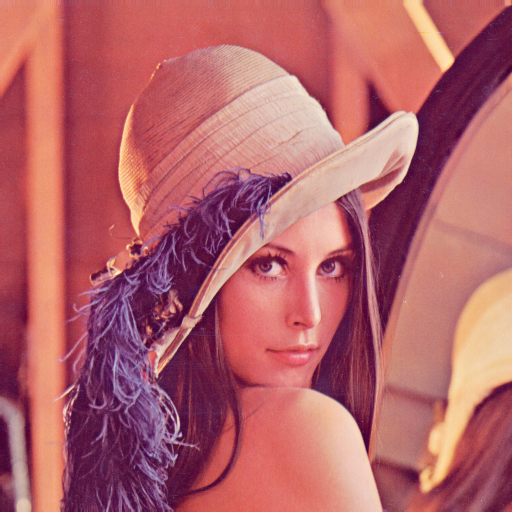
\includegraphics[width=0.45\textwidth]{../images/lena1.png}}
\subfigure[\label{fig:lena2}]{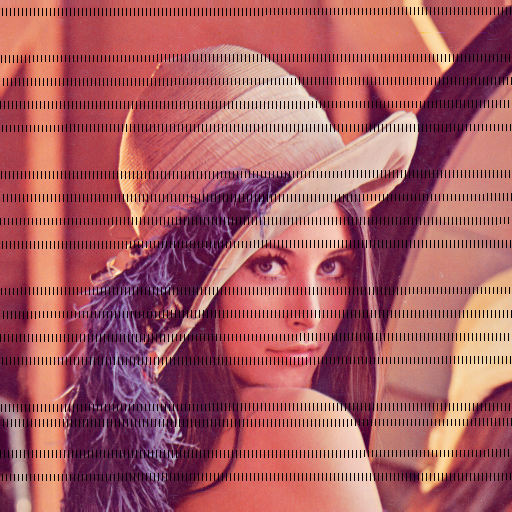
\includegraphics[width=0.45\textwidth]{../images/lena2.png}}
	\caption{Immagine sorgente e immagine ricevuta.}
\end{figure}

\begin{figure}[b]
\centering
\subfigure[\label{fig:lena3}]{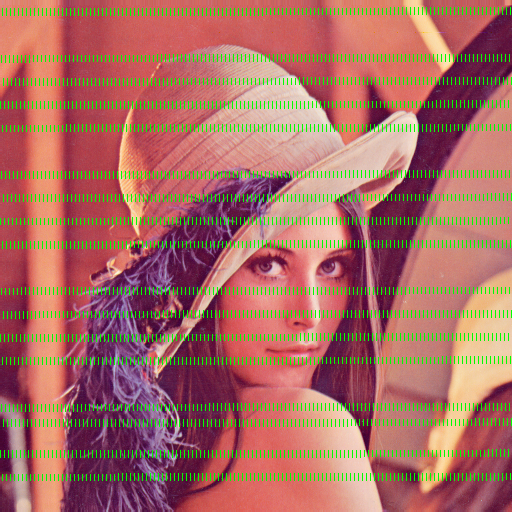
\includegraphics[width=0.45\textwidth]{../images/lena3.png}}
\subfigure[\label{fig:lena4}]{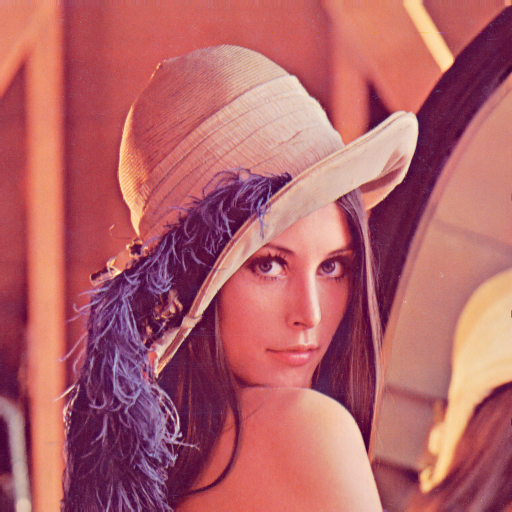
\includegraphics[width=0.45\textwidth]{../images/lena4.png}}
	\caption{Evidenziazione dei pixel mancanti e immagine dopo l'interpolazione.}
\end{figure}

La figura \ref{fig:lena2} mostra la totalità di pixel correttamente
ricevuti. Nella figura \ref{fig:lena3}, in verde, è possibile notare i pixel
mancanti. La figura \ref{fig:lena4} presenta leggerissime imperfezioni
(praticamente invisibili) dovute esclusivamente alla perdita dei pixel associati ai descrittori persi durante il trasferimento. In tali zone dell'immagine è stato eseguito l'algoritmo di interpolazione.

In figura \ref{fig:occhi}, invece, è mostrato il funzionamento del codec grafico
nel caso in cui viene richiesta la trasmissione a bassa qualità. \`E illustrato
in dettaglio il funzionamento dell'algoritmo di interpolazione. I pixel non correttamente ricevuti vengono sostituiti con pixel predetti in base alle componenti di
colore dei pixel vicini. L'opacità accentuata di alcuni pixel è dovuta alla
quantità non sufficiente di pixel validi su cui effettuare la previsione.

\begin{figure}[ht]

\includegraphics[width=0.90\textwidth]{../images/occhi.png}
\centering \caption{Particolare dettaglio sul risultato dell'interpolazione.}
	\label{fig:occhi}
\end{figure}
Come è possibile notare, la trasmissione dati presa in esame ha prodotto una
quantità molto esigua di pixel validi (caso peggiore), tuttavia è ancora
possibile scorgere l'immagine originale ed il suo contenuto visivo. L'immagine sorgente possiede
una larghezza di 512 pixel, tale dimensione (multipla del numero di flussi
trascurati durante il trasferimento) fa sì che i pixel mancanti si dispongano
secondo linee verticali. \`E possibile apprezzare la robustezza del
sistema di trasmissione e di codifica/decodifica di MDSP che mantiene il contenuto informativo di un file
grafico nonostante la quantità di informazioni richiesta per la sua descrizione
sia fortemente insufficiente ed in parte errata.


\section{Esempio codec testuale}
\label{sec:esempio_codec}
Quì di seguito si procede alla descrizione dei principali comandi in linguaggio
C++ che formano una funzione di codifica MDC compatibile.

\begin{notabene}
La dicitura \textit{flow} è viene usata con il significato di
`\emph{Descrizioni}'. Tale variazione rispetto alla nomenclatura presente in
letteratura è stata adottata al fine di evitare la possibile confusione dovuta
alla somiglianza dei termini `\emph{Descrizioni}' e `\emph{Descrittori}'. In seguito, quindi, la parola `\emph{Flussi}' è da intendersi con il significato di `\emph{Descrizioni}'.
\end{notabene}

\begin{itemize}
 \item \begin{code}
Uint32 flow\_dimension = (stream\_size/m\_flows\_number)+1;\\
Uint32 descriptors\_number = \\(Uint32)ceil(((double)flow\_dimension)/((double)m\_preferred\_payload\_size));\\
Uint16 max\_payload\_size = (flow\_dimension/descriptors\_number)+1;\\
\end{code}

Innanzitutto è necessario calcolare dimensione dei flussi, numero di flussi e
descrittori. Il numero di descrittori da generare viene calcolato tenendo conto
della \emph{dimensione preferita}, impostata dall'utente tramite linea di
comando con il parametro \texttt{--payload} (vedi paragrafo \ref{sec:opzioni});
viene altresì utilizzata la dimensione predefinita nel caso non venga impostato alcun parametro. Si tratta di un parametro \emph{preferito} poiché il codec ha l'obiettivo di generare \emph{N} flussi sui quali devono essere distribuiti in modo possibilmente eguale i dati del file sorgente. Il parametro \textit{max\_payload\_size} ha quindi il compito di bilanciare il carico tra i flussi.

 \item \begin{code}
md\_stream->init(stream->compute\_hash\_md5(), m\_flows\_number, descriptors\_number);\\
\end{code}
Si inizializza un oggetto di tipo \textit{md\_stream} (Multiple Description
Stream) con un codice hash MD5 che viene calcolato a partire dal file sorgente su disco, si specificano altresì il numero di flussi e di descrittori.

 \item \begin{code}
Descriptor* descriptor = new Descriptor();\\
descriptor->set\_stream\_id(md\_stream->get\_stream\_id());\\
descriptor->set\_flow\_id(i);\\
descriptor->set\_sequence\_number(j);\\
descriptor->set\_codec\_name(string("text"));\\
\end{code}
L'n-esimo descrittore viene inizializzato in memoria e viene impostato il
parametro \textit{stream\_id} copiandolo da quello generato dal file sorgente su disco. Successivamente viene inserito il numero di flusso e sequenza che lo contraddistingue tra tutti gli altri descrittori del file. Il numero di sequenza viene incrementato per ogni nuovo descrittore ed è unico all'interno di un flusso. Con esso si può distinguere un descrittore all'interno di un flusso, la coppia di parametri (\textit{flow\_id}, \textit{descriptor}) individua un descrittore e lo distingue da tutti gli altri nell'ambito dell'intero file. Infine viene impostato il nome del codec che contrassegna ogni descrittore. Tale nome ha lo scopo di identificare, in fase di decodifica, il tipo di dati contenuti all'interno di un descrittore.

 \item \begin{code}
TextCodecParameters* tcp = new TextCodecParameters();\\
descriptor->set\_codec\_parameter(tcp);\\
\end{code}
Viene inizializzato un oggetto \textit{tcp} di tipo TextCodecParameters che
contiene i parametri del codec. Poichè il testo semplice non possiede parametri significativi, tale oggetto viene inizializzato vuoto. Dopo la creazione, viene anch'esso associato al descrittore.

 \item \begin{code}
MemDataChunk payload;\\
Uint64 k;\\
for (k=0; k<max\_payload\_size; k++)\\
	if (offset+i+k+m\_flows\_number < stream\_size)\\
		payload += \&stream->get\_data(offset+i+(k*m\_flows\_number), 1);\\
offset += m\_flows\_number*k;\\
descriptor->set\_payload(payload);\\
\end{code}
Terminata la fase di preparazione del descrittore, si passa alla fase del
riempimento con i dati prelevati dal file sorgente su disco. Viene inizializzata
in memoria una struttura dati che consente di caricare porzioni di file da disco.
Con un ciclo for vengono prelevati i caratteri dal file sorgente e inseriti nella
struttura dati creata. Il parametro \textit{offset} e la formula che lo contiene
consentono di rispettare i vincoli di codifica, si tratta dei vincoli illustrati
in appendice \ref{sec:spec-text}. Finita la preparazione del payload,
quest'ultimo viene accodato al descrittore che adesso risulterà completo.

 \item \begin{code}
md\_stream->set\_descriptor(descriptor);\\
\end{code}
Infine, l'N-esimo descrittore viene accodato al Multiple Description Stream per poter essere inviato.
\end{itemize}
In appendice è riportato il codice completo della funzione di codifica testuale
appena descritta.


\section{Decodifica:}

\begin{itemize}
 \item \begin{code}
Uint8 flows\_number = md\_stream->get\_flows\_number();\\
Uint32 sequences\_number = md\_stream->get\_sequences\_number();\\
\end{code}
Dopo aver controllato che il Multiple Description Stream non sia vuoto, si creano due variabili contenenti il numero di flussi e delle sequenze dello stream (si ricordi che rispettivamente indicano il numero di descrizioni dello stream e di descrittori di ogni descrizione).

 \item \begin{code}
payload\_size = descriptor->get\_payload\_size();\\
if (md\_stream->is\_valid(descriptor->get\_flow\_id(), descriptor->get\_sequence\_number()))\{
	(*dc) += (descriptor->get\_payload());\\
	taken\_stream.resize(flows\_number*sequences\_number*(payload\_size+1));\\
	Uint8 current\_received\_data;\\
	Uint64 k;\\
	for (k=0; k<payload\_size; k++) \{\\
		dc->extract\_head(current\_received\_data);\\
		if (current\_received\_data != 0) \{\\
			Uint64 locate\_position = offset+i+(k*flows\_number);\\
			taken\_stream[locate\_position] = current\_received\_data;\\
			if (locate\_position > max\_dimension)\\
			max\_dimension = locate\_position;\\
		\}\\
	\}\\
	offset += flows\_number*k;\\
\}\\
\end{code}
La porzione di codice che si sta per analizzare è di fondamentale importanza.
Tutte le operazioni vengono effettuate sul descrittore correntemente
selezionato, quindi si eviterà di ripeterlo. Innanzitutto viene memorizzata la
dimensione del payload, tale dimensione è costante e può variare esclusivamente
per l'ultimo descrittore di un flusso.
\begin{notabene}
Non ha senso effettuare paragoni tra descrittori appartenenti a flussi diversi, in quanto non sono in alcun modo correlati.
\end{notabene}
Se il descrittore corrente viene ritenuto valido all'interno del Multiple
Description Stream si passa alla decodifica. Viene prelevato il payload e
trasferito in una struttura dati in memoria (Memory DataChunk). Il contenitore temporaneo dello stream decodificato viene ridimensionato per contenere (potenzialmente) tutti i payload provenienti da tutti i descrittori. \`E possibile raggiungere la dimensione massima esclusivamente nel caso in cui non vi sia alcun errore di trasmissione. Successivamente si prelevano le singole lettere dalla struttura dati in memoria. Se la i-esima lettera estratta ha un codice ascii diverso da `\emph{0}' si passa al calcolo della sua posizione assoluta all'interno dello stream finale (decodificato) e al posizionamento del carattere corrente in tale posizione. Infine viene aggiornato un contatore che tiene conto della massima posizione raggiunta in tale fase. Tale contatore servirà successivamente, pertanto il suo significato verrà descritto in seguito.

 \item \begin{code}
else\{\\
	Uint64 k;\\
	for (k=0; k<payload\_size; k++) \{\\
		Uint64 locate\_position = offset+i+(k*flows\_number);\\
		taken\_stream[locate\_position] = ' ';\\
	\}\\
	offset += flows\_number*k;\\
\}\\
\end{code}
Nel caso in cui il descrittore corrente, per qualunque motivo, non sia valido vengono calcolate tutte le posizioni nello stream finale relative alle lettere contenute nel suo payload che sono considerate perse. Al loro posto vengono sostituiti dei caratteri `\emph{spazio}'.

 \item \begin{code}
MemDataChunk* taken\_dc = new MemDataChunk();\\
Uint8* temp\_container = new Uint8[max\_dimension+1];\\
for (Uint64 i=0; i<max\_dimension+1; i++)\\
	temp\_container[i] = taken\_stream[i];\\
taken\_dc->append\_data(max\_dimension+1, temp\_container);\\
\end{code}
Terminata l'analisi di tutti i descrittori validi si devono rendere
comprensibili (oltre che validi) i dati ricevuti. Si crea una lista di
puntatori a locazioni da 8 bit (quindi caratteri) di dimensione pari
all'estensione della porzione di stream decodificata correttamente. Se tutti i
descrittori analizzati si sono rivelati validi tale dimensione coinciderà con
quella dello stream inviato dalla sorgente. Se, invece, saranno presenti errori tale dimensione sarà minore di quella originale. La dimensione della porzione di stream valido è di fondamentale importanza poiché segnerà il limite entro il quale ogni puntatore della lista `punta' ad un valore realmente utile della memoria e non ad un valore impredicibile. Si procede successivamente al travaso dei dati dallo stream temporaneo alla lista di puntatori. L'ultima istruzione inserisce nell'apposita struttura dati in memoria il contenuto della lista di puntatori.

 \item \begin{code}
stream->set\_data(*taken\_dc);\\
\end{code}
Il comando finale riempie lo stream con le lettere presenti nella struttura dati appena preparata.
\end{itemize}
In appendice \ref{cap:decode} è riportato il codice completo della funzione di
codifica testuale appena descritta.

